\chapter{Hypothèses de travail}

\section{ARTrack}

L’ARTrack  pour Advanced Realtime Tracking est un ensemble de caméra infrarouge développé par la société Vicon. Ces caméras fonctionnent grâce à des marqueurs. Il est possible de traquer avec précision n’importe quel élément équipé de trackers. 

\begin{figure}[!ht]
	\center	
	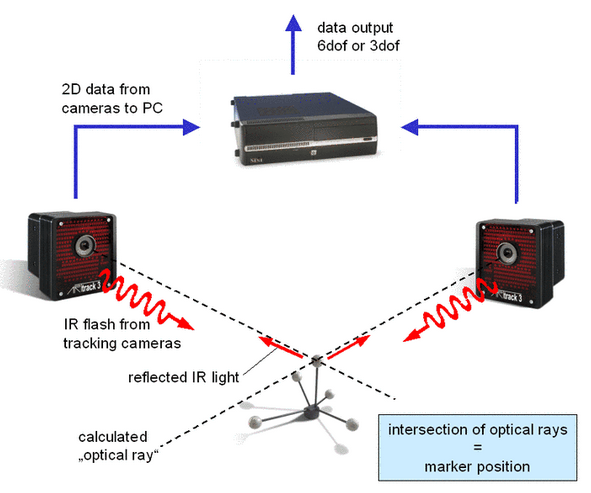
\includegraphics[scale=0.5]{image/artrack.png}
	\caption{ARTrack}
\end{figure}

Cette solution présente plusieurs avantages. Premièrement la précision, les ARTracks sont des caméras permettant de tracker n’importe quoi avec une grande précision. Tracker la position de la main de l’utilisateur ainsi que le support physique seront suivis avec énormément de précision. Une pièce configurée avec un ensemble de caméra ARTrack pourrait permettre de résoudre les problèmes de précision mais également d’obstruction.

Cependant nous souhaitons mettre en oeuvre une solution disponible au grand public. Les ARTracks étant un équipement coûteux et complexe dans son installation ainsi que dans sa  calibration, cette technologie ne peut pas utilisé dans le cadre d’une application grand public.

\section{Tag}

Pour tracker facilement un objet, nous pouvons lui ajouter des QR Codes. Les QR Codes sont un type de codes barres à deux dimensions. Il est aujourd’hui l’un des codes bidimensionnels les plus utilisés. Il sont en effet utilisés pour rediriger vers un site internet ou encore pour afficher du contenu multimédia.

\begin{figure}[!ht]
	\center	
	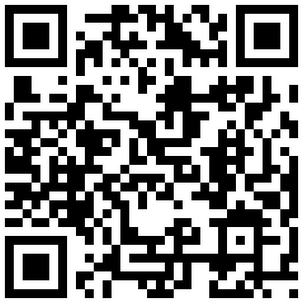
\includegraphics[scale=0.25]{image/qrcode.png}
	\caption{QrCode}
\end{figure}

L’utilisation des QR Codes permettrait donc de différencier les objets physiques lambda et le support physique sélectionné pour interagir. De plus en utilisant les QR Code il serait possible d’utiliser différents types d’interaction en fonction du support sur lequel on plaque le QR Code. Par exemple, on pourrait définir un QR Code pour un bloc note et, dès le début de l’interaction, un éditeur de texte pourrait s’ouvrir pour prendre en note l’écriture de l’utilisateur. Cela permettrait également d’obtenir la position exacte et l’orientation de l’objet. 

Cependant cette solution ne sera pas retenue car nous souhaitons une application grand public sans aucune contrainte, cf pose des QR Code sur les supports.

\section{Solution multi-Kinect}

Étant donné que notre problème principale est que, lorsque le support physique est à la verticale, le champ de vision de la Kinect est obstrué par celui-ci. On peut donc penser à utiliser plusieurs Kinects pour éviter les angles mort. 

La logique est simple, l’utilisateur se met face à la Kinect principale pour que celle-ci l’identifie et analyse ses mouvements. Une fois que la Kinect principale a trouvé l’emplacement de l’utilisateur, la deuxième Kinect analyse les mouvements de celui-ci et les données des deux Kinects sont fusionnés pour plus de précision. 

Grâce à cette deuxième Kinect, lorsqu’un objet est présent entre l’utilisateur et la Kinect ou lorsque le support physique est vertical, la deuxième Kinect permet de récupérer quand même le mouvement et donc l’application fonctionne toujours.
	
Le problème est que l’utilisation de deux Kinect en stéréovision est compliqué et que cela nécessite une bonne configuration des Kinect. Un calibrage important est nécessaire .


\section{Kinect en hauteur}

Une possibilité pour pouvoir éviter l’occlusion causée par le support physique serait de mettre la caméra Kinect en hauteur. Celle-ci bénéficiera d’un point de vue qui permettra une plus grande liberté dans le placement du support physique par l’utilisateur.

\begin{figure}[!ht]
	\center	
	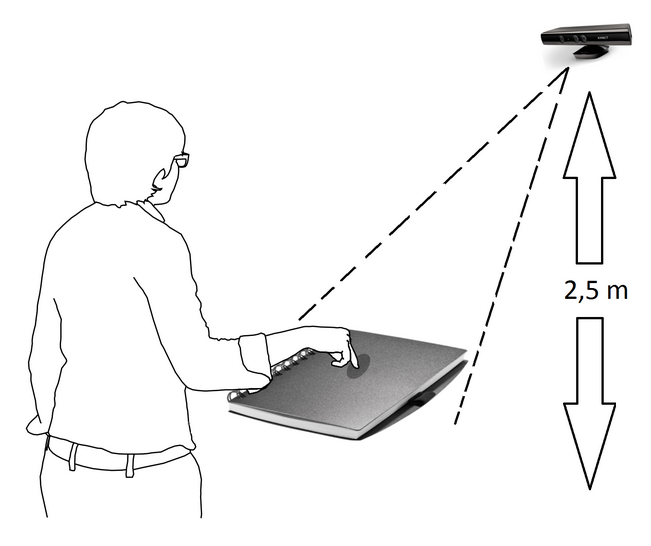
\includegraphics[scale=0.25]{image/result.png}
	\caption{Proposition de placement de la Kinect}
\end{figure}

Certes, cette solution n’est pas idéale dans le sens que, l’occlusion sera toujours possible puisque nous restons dans un environnement visuel à deux dimensions. Elle reste pour autant la solution la plus abordable pour le grand public puisque, une et une seule Kinect est nécessaire ce qui facilite l’intégration. Cependant certaines conditions d’installations seront à respecter, tels que la hauteur de la Kinect ou encore son angle d’orientation.
